% !TEX TS-program = lualatex
% !TEX encoding = UTF-8

% This is a simple template for a LuaLaTeX document using gregorio scores.

\documentclass[letterpaper,12pt]{book} % use larger type; default would be 10pt

\input{header.inc}

\geometry{letterpaper,outer=0.4in,inner=0.9in,top=0.5in,bottom=0.8in}

\begin{document}
\printtitle{Reception of a Bishop}

\large
Although these ceremonies are available here if needed, in most cases they will not
apply. These rites apply when the bishop is diocesan and paying a pastoral visit.

\bigskip

\emph{On the Bishop's arrival, the Priest presents him with a crucifix to be
kissed; the Cantors then intone the following Antiphon~:}

\bigskip

{
	\garamondbig
	\greannotation{Ant.}
	\greannotation{1.}
	\gregorioscore{149_1840_an--sacerdos_et_pontifex_sic--solesmes}
}

%\large
%\garamond

\emph{The following Responsory may also be sung~:}
\bigskip

{
	\garamondbig
	\greannotation{Resp.}
	\greannotation{8.}
	\gregorioscore{149_1841_re--ecce_sacerdos--solesmes}
}

\smallskip

\begin{centering}

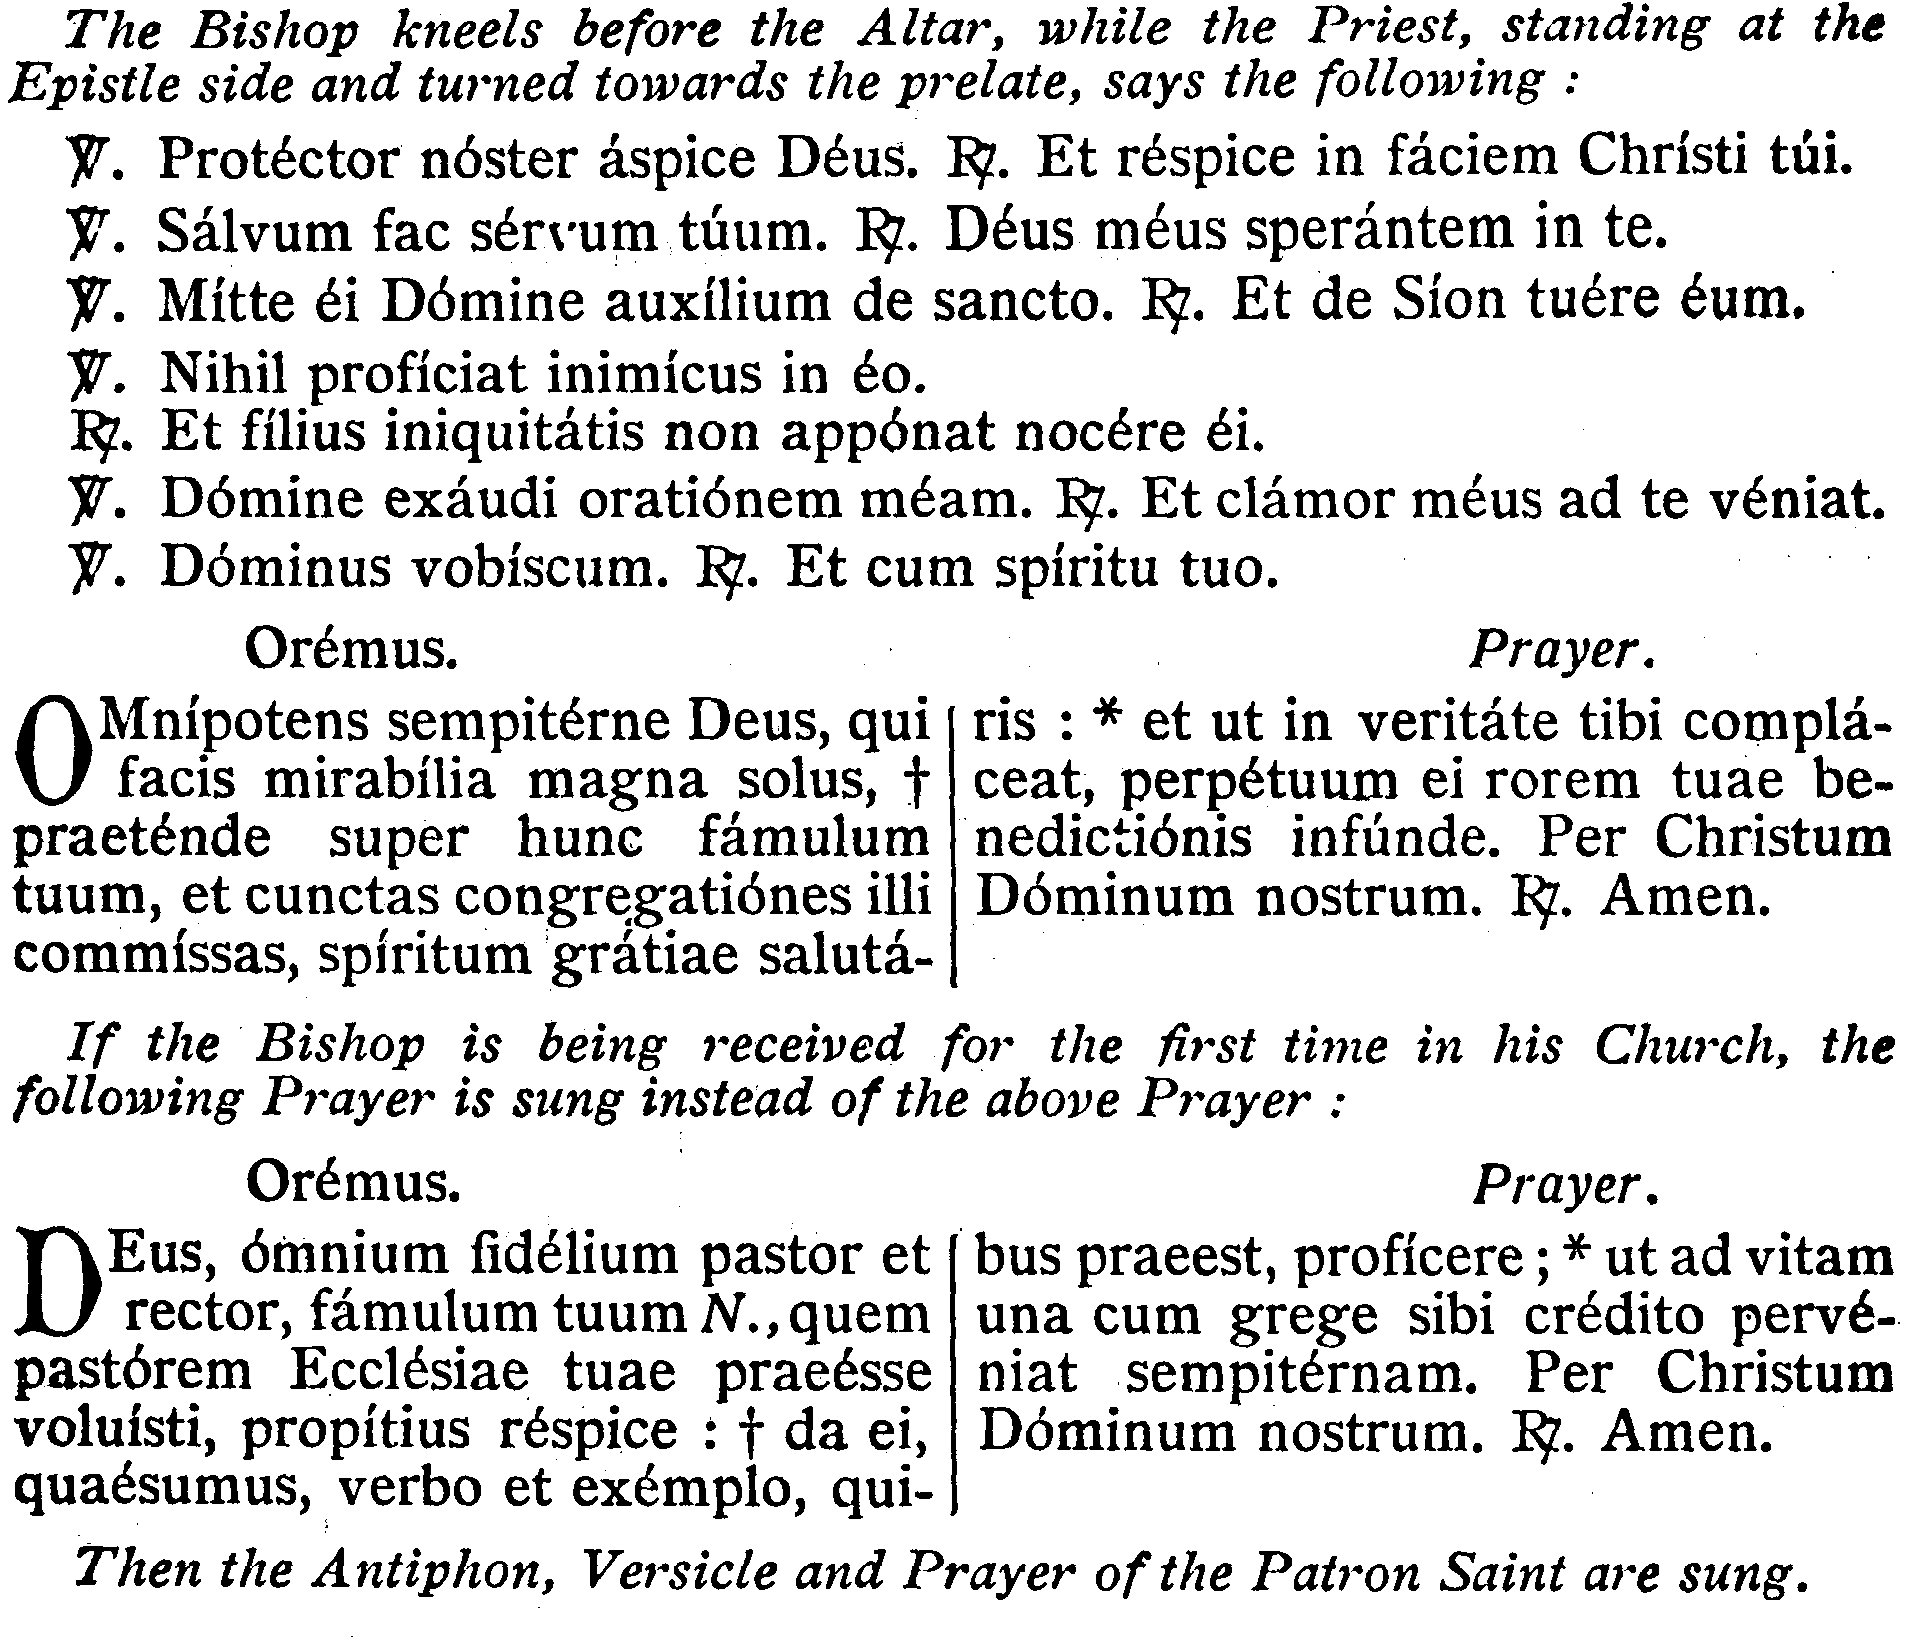
\includegraphics[width=0.95\textwidth]{151-1.png}

\end{centering}


\printtitle{Administration of Confirmation}

\begin{centering}

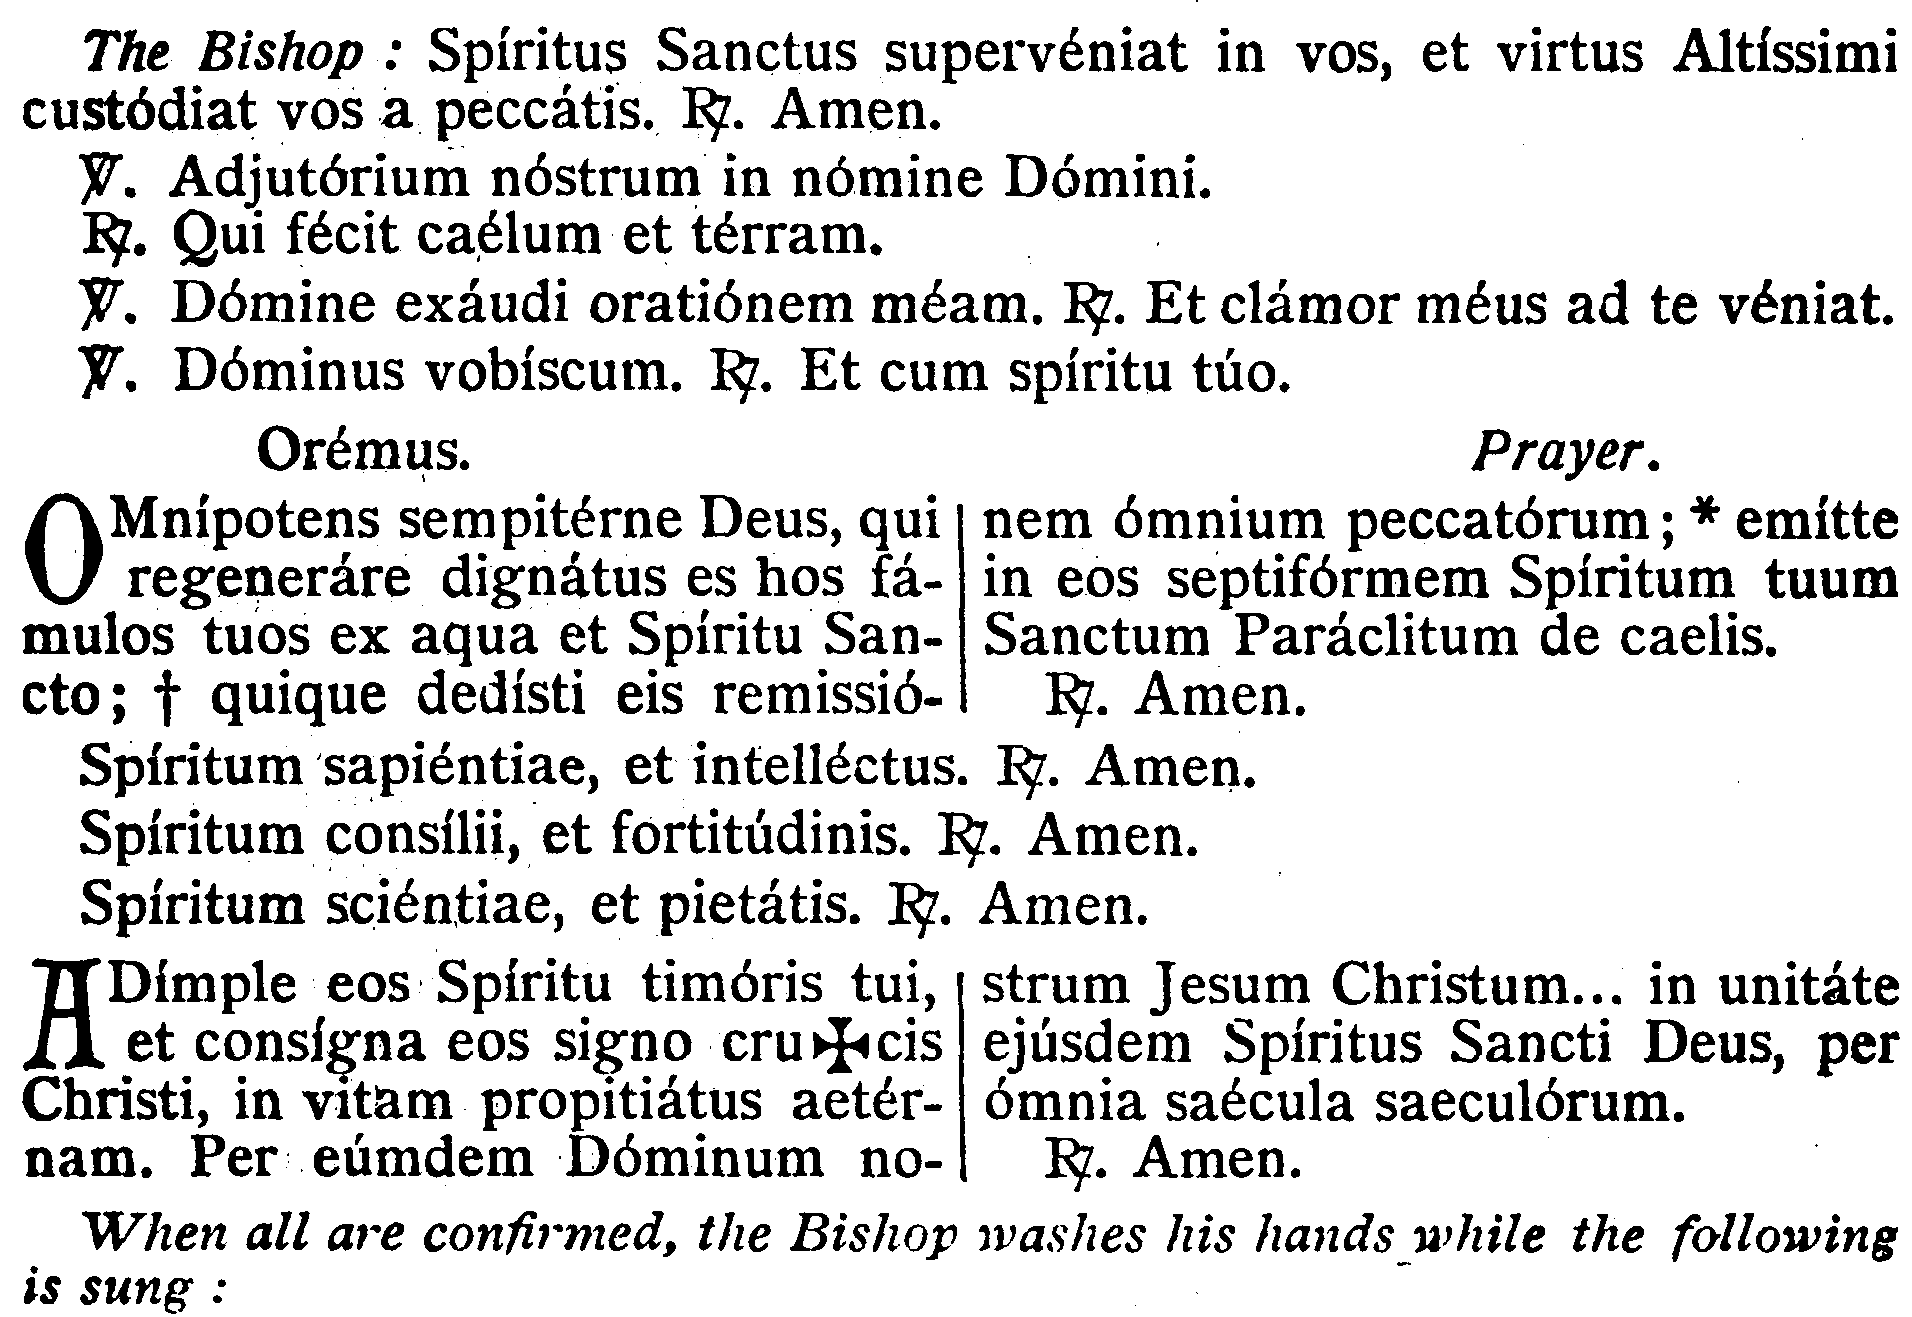
\includegraphics[width=\textwidth]{151-2.png}

\end{centering}

\bigskip

{
	\garamondbig
	\greannotation{Ant.}
	\greannotation{8. c}
	\gregorioscore{151_1844_an--confirma_hoc_deus--solesmes}
}

\begin{centering}

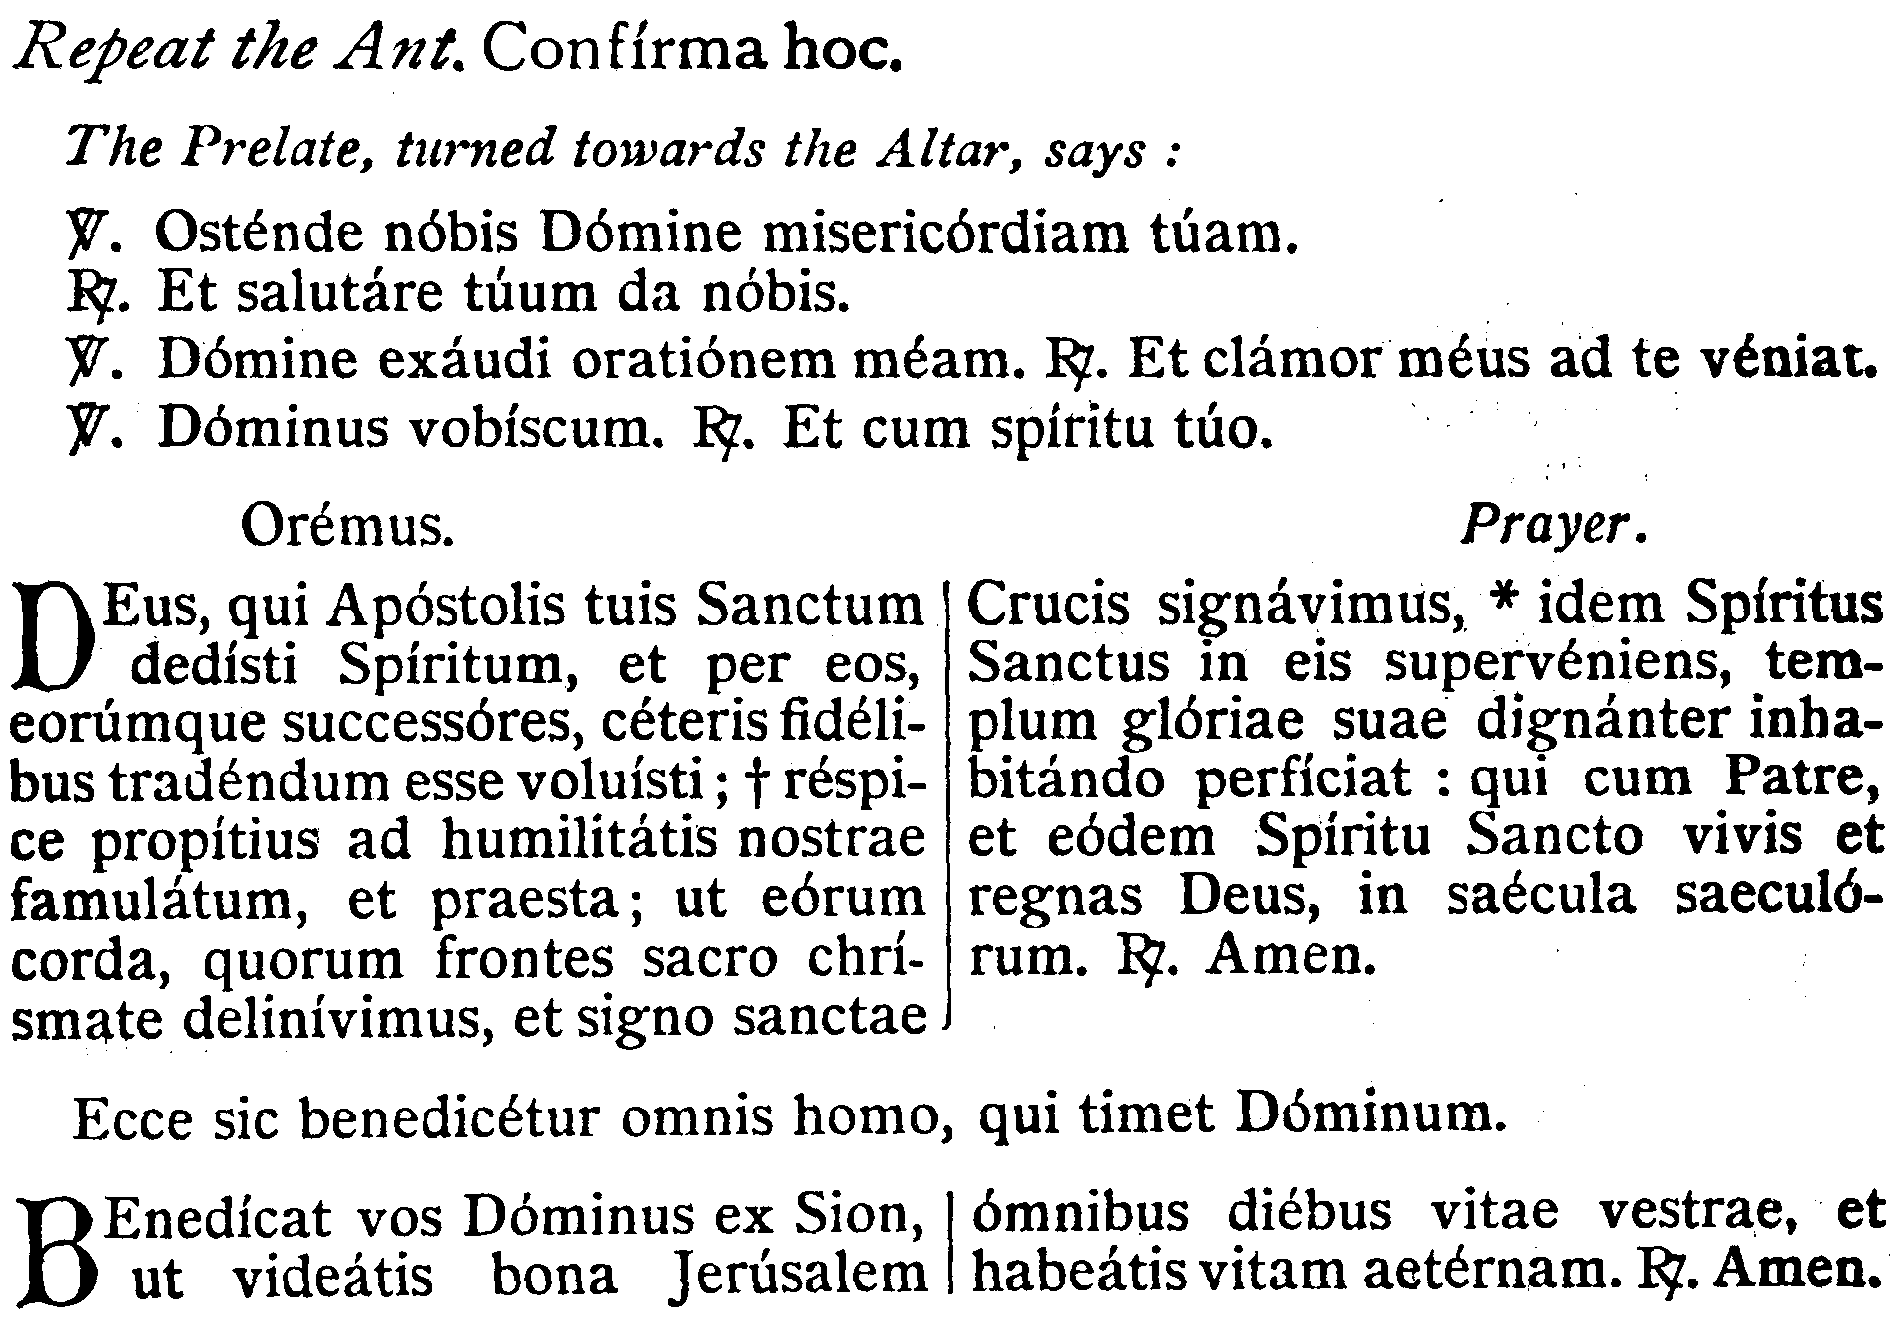
\includegraphics[width=\textwidth]{152-1.png}

\end{centering}

\bigskip

%\large
%\garamond

The gist of the ceremony is:
\begin{itemize}
\item Sing a processional such as Come, Holy
Ghost as the Bishop enters the church.
\item Bishop intones the Veni Creator. After the
versicle, response, and prayer for the
Hymn, the versicles and prayers above
are sung. There may be a discourse
before the sacrament is administered.
\item During the confirmations, any suitable
music, organ or sung piece (e.g. Veni
Sancte Spiritus) may be done.
\item Following the administration of the
sacrament. Confirma Hoc is sung during
the ablution of the Bishop.
\item Sing a recessional such as Come, Holy
Ghost or any other suitable piece as the
Bishop leaves the sanctuary.
\end{itemize}

\bigskip

\printtitle{Benediction Chants}

{
	\garamondbig
	\#1

	\greannotation{Hymn.}
	\greannotation{8.}
	\gregorioscore{153_hy--o_salutaris_hostia_i--solesmes}

	\bigskip
	\#2

	\greannotation{Hymn.}
	\greannotation{7.}
	\gregorioscore{153_2_hy--o_salutaris_hostia_ii--solesmes}

	\bigskip
	\#1

	\greannotation{Hymn.}
	\greannotation{3.}
	\gregorioscore{154_hy--tantum_ergo--solesmes}

	\bigskip
	\bigskip
	\#2

	\greannotation{Hymn.}
	\greannotation{1.}
	\gregorioscore{155_hy--tantum_ergo_ii--solesmes}

	\bigskip
	\vfill
	\pagebreak
	\#3

	\greannotation{Hymn.}
	\greannotation{5.}
	\gregorioscore{156_hy--tantum_ergo_iii--solesmes}

	\bigskip
	\#4

	\greannotation{Hymn.}
	\greannotation{5.}
	\gregorioscore{157_hy--tantum_ergo_i--solesmes}
}

\bigskip

\begin{centering}

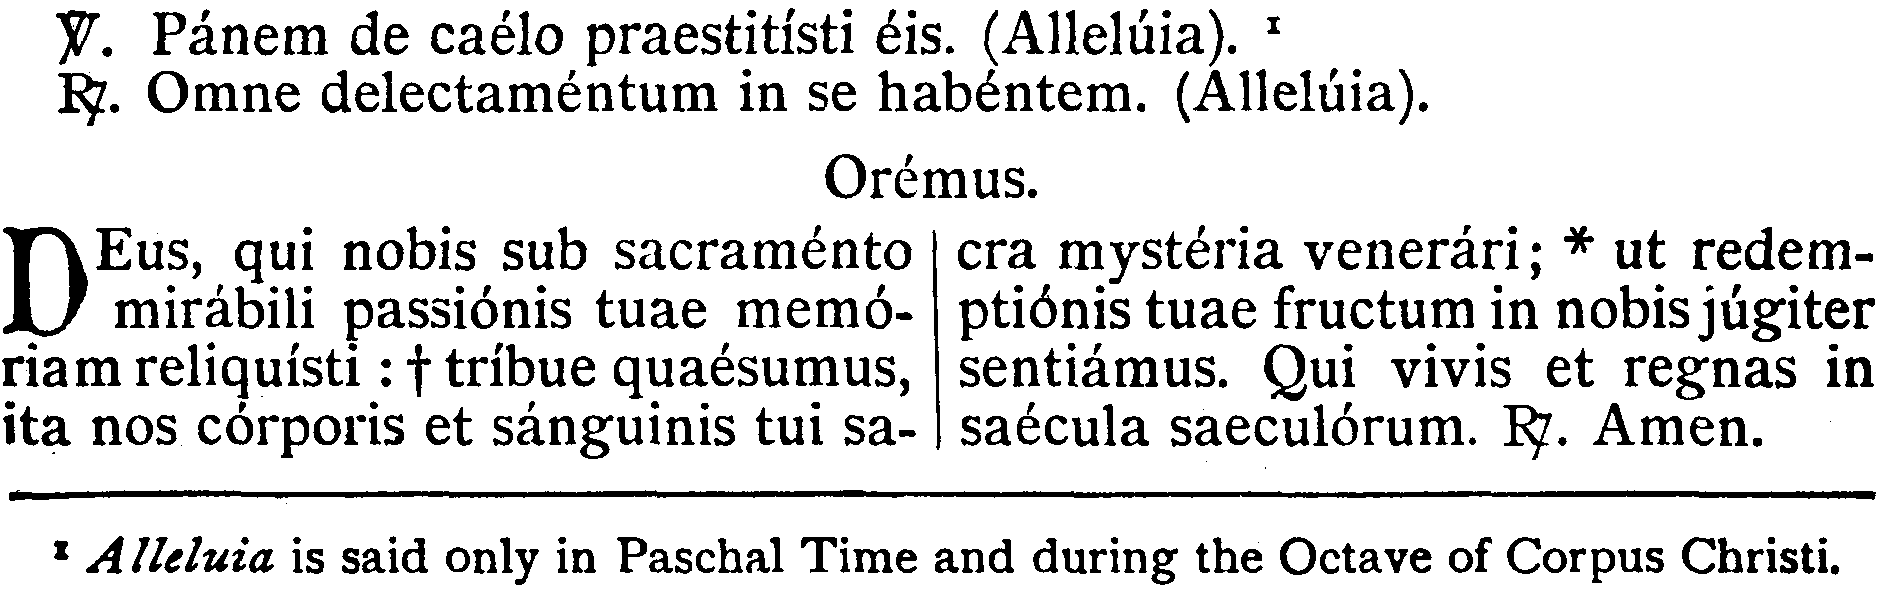
\includegraphics[width=\textwidth]{158-1.png}

\end{centering}

\bigskip
\clearpage

\begin{centering}

\vspace*{\fill}

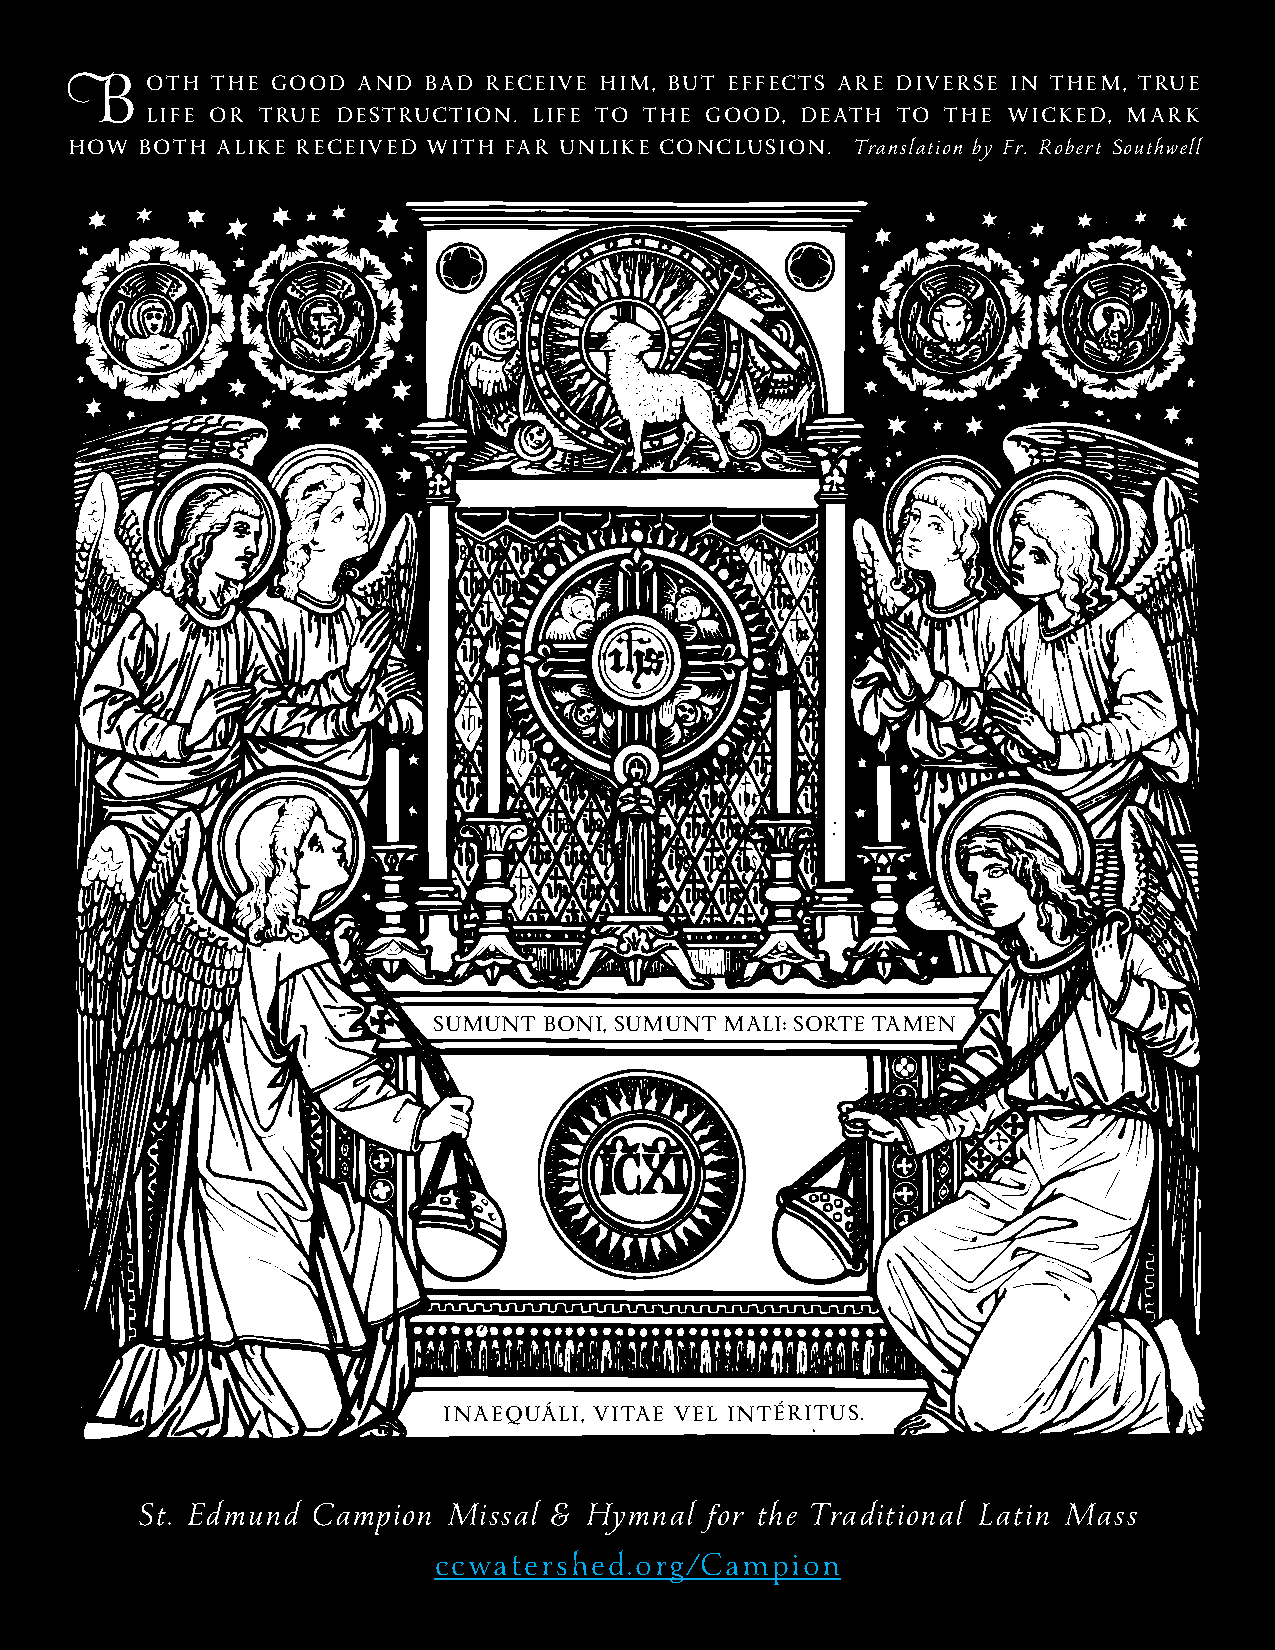
\includegraphics[clip,trim=0.379in 1.318in 0.378in 1.242in,width=\textwidth]{../158_clipart.pdf}

\vfill

\end{centering}

\pagebreak

{
	\garamondbig
	\greannotation{Ant.}
	\greannotation{5.}
	\gregorioscore{158_an--adoremus_in_aeternum_i--solesmes}
}

\end{document}